\documentclass[12pt]{article}
\usepackage[spanish]{babel}
\usepackage[utf8]{inputenc}
\usepackage{graphicx}
\usepackage{geometry}
\geometry{margin=2cm, headheight=14.5pt}
\usepackage{fancyhdr}
\usepackage{color}
\usepackage{titlesec}
\usepackage{setspace}
\usepackage{hyperref}
\usepackage{longtable}
\usepackage{booktabs}
\usepackage{listings}
\usepackage{enumitem}
\onehalfspacing
% Evitar que LaTeX estire verticalmente la página y genere espacios en blanco grandes
\raggedbottom

% Definición de colores
\definecolor{uvred}{RGB}{180,0,0}

% Configuración de títulos
\titleformat{\section}{\normalfont\Large\bfseries\color{uvred}}{\thesection}{1em}{}
\titleformat{\subsection}{\normalfont\large\bfseries\color{uvred}}{\thesubsection}{1em}{}
\titleformat{\subsubsection}{\normalfont\normalsize\bfseries\color{uvred}}{\thesubsubsection}{1em}{}

% Configuración de encabezados y pies de página
\pagestyle{fancy}
\fancyhf{}
\fancyhead[L]{Universidad del Valle}
\fancyhead[C]{Informe Técnico BrainBlitz}
\fancyhead[R]{Ervin Caravalí Ibarra}
\renewcommand{\headrulewidth}{0.4pt}

% Títulos con color suave
\definecolor{uvred}{RGB}{180,0,0}
\titleformat{\section}{\normalfont\Large\bfseries\color{uvred}}{\thesection}{1em}{}
\titleformat{\subsection}{\normalfont\large\bfseries\color{uvred}}{\thesubsection}{1em}{}

% Portada
\begin{document}
\begin{titlepage}
    \begin{center}
        % Encabezado institucional
        \vspace*{-1cm}
        {\Large UNIVERSIDAD DEL VALLE}\\[0.3cm]
        {\large FACULTAD DE INGENIERÍA}\\[0.3cm]
        {\large ESCUELA DE INGENIERÍA DE SISTEMAS Y COMPUTACIÓN}\\[2cm]
        
        % Logo
        
\includegraphics[width=0.25\textwidth]{Universidad-del-Valle.jpg}\\[1.5cm]
        
        % Título del proyecto
        {\Huge\bfseries INFORME TÉCNICO:\\[0.3cm]
        PROYECTO BRAINBLITZ}\\[0.8cm]
        {\Large\bfseries Desarrollo de Accesibilidad en\\
        Juegos de Trivia Multijugador}\\[1.5cm]
        
        % Información del curso
        {\large\bfseries Curso}\\[0.3cm]
        {\large PROYECTO INTEGRADOR II GRUPO-01}\\[1.5cm]
        
        % Información del autor y docente
        \begin{tabular}{rl}
            \textbf{Autor:} & Ervin Caravalí Ibarra \\[0.3cm]
            \textbf{Código:} & 1925648 \\[0.3cm]
            \textbf{Docente:} & CARLOS MAURICIO GAONA CUEVAS \\[0.3cm]
        \end{tabular}\\[1cm]
        
        % Fecha
        {\large Santiago de Cali}\\[0.3cm]
        {\large Octubre 27, 2025}
        
        \vfill
    \end{center}
\end{titlepage}

% Índice automático
\tableofcontents
\newpage

% Estructura del documento
\section*{Estructura del documento}
Este informe técnico está organizado en las siguientes secciones principales:

\begin{enumerate}
    \item \textbf{Introducción}: Contexto y objetivos del proyecto
    \item \textbf{Marco teórico y tecnologías}: Base teórica y stack tecnológico
    \item \textbf{Arquitectura y diseño}: Estructura y patrones de diseño
    \item \textbf{Implementación}: Detalles de desarrollo e integración
    \item \textbf{Desarrollo y documentación de prompts}: Prompts de IA utilizados
    \item \textbf{Plan de pruebas}: Estrategias y resultados de testing
    \item \textbf{Resultados y métricas}: Evaluación del proyecto
    \item \textbf{Conclusiones}: Reflexiones y aprendizajes
    \item \textbf{Referencias}: Fuentes y documentación
    \item \textbf{Anexos}: Documentación adicional y recursos
\end{enumerate}

\newpage

% Introducción
\section{Introducción}
El presente informe documenta el desarrollo técnico y funcional del proyecto BrainBlitz, un sistema de trivia multijugador enfocado en accesibilidad para personas con discapacidades visuales. El proyecto integra tecnologías modernas como Node.js, Express, React, Firebase, Docker y Render, y se ha guiado por metodologías ágiles y criterios de evaluación académica. Se abordan los objetivos, arquitectura, implementación, integración de IA, despliegue y resultados, siguiendo la rúbrica de evaluación del curso.

% Descripción general del proyecto
\section{Descripción general del proyecto}
BrainBlitz es una plataforma de juego de trivia multijugador que permite la participación inclusiva de usuarios con diferentes capacidades visuales. El sistema gestiona usuarios, partidas, preguntas y respuestas, integrando funcionalidades de accesibilidad como modo de voz, lectura de preguntas mediante TTS, y registro de preferencias. El flujo de información se basa en una arquitectura cliente-servidor, con operaciones CRUD sobre usuarios, partidas y preguntas, y una gestión eficiente de proyectos y tareas.

% Objetivos del proyecto
\section{Objetivos del proyecto}
\subsection{Objetivo general}
Desarrollar un sistema de trivia multijugador accesible, que permita la participación plena de usuarios con discapacidades visuales mediante tecnologías de voz y accesibilidad.

\subsection{Objetivos específicos}
\begin{itemize}
    \item Implementar funcionalidades de accesibilidad visual y modo de voz en el registro y uso del sistema.
    \item Integrar tecnologías de Text-to-Speech y reconocimiento de voz para la interacción en el juego.
    \item Desplegar el sistema en infraestructura cloud, asegurando escalabilidad y disponibilidad.
\end{itemize}

% Arquitectura del sistema
\section{Arquitectura del sistema}
El sistema sigue un diseño cliente-servidor, con una API RESTful en el backend y una SPA en el frontend. La arquitectura REST permite la interacción eficiente entre componentes, y el flujo de datos se gestiona mediante endpoints y WebSockets para partidas en tiempo real. El siguiente diagrama BPMN ilustra el flujo principal de procesos:

\begin{figure}[h!]
    \centering
    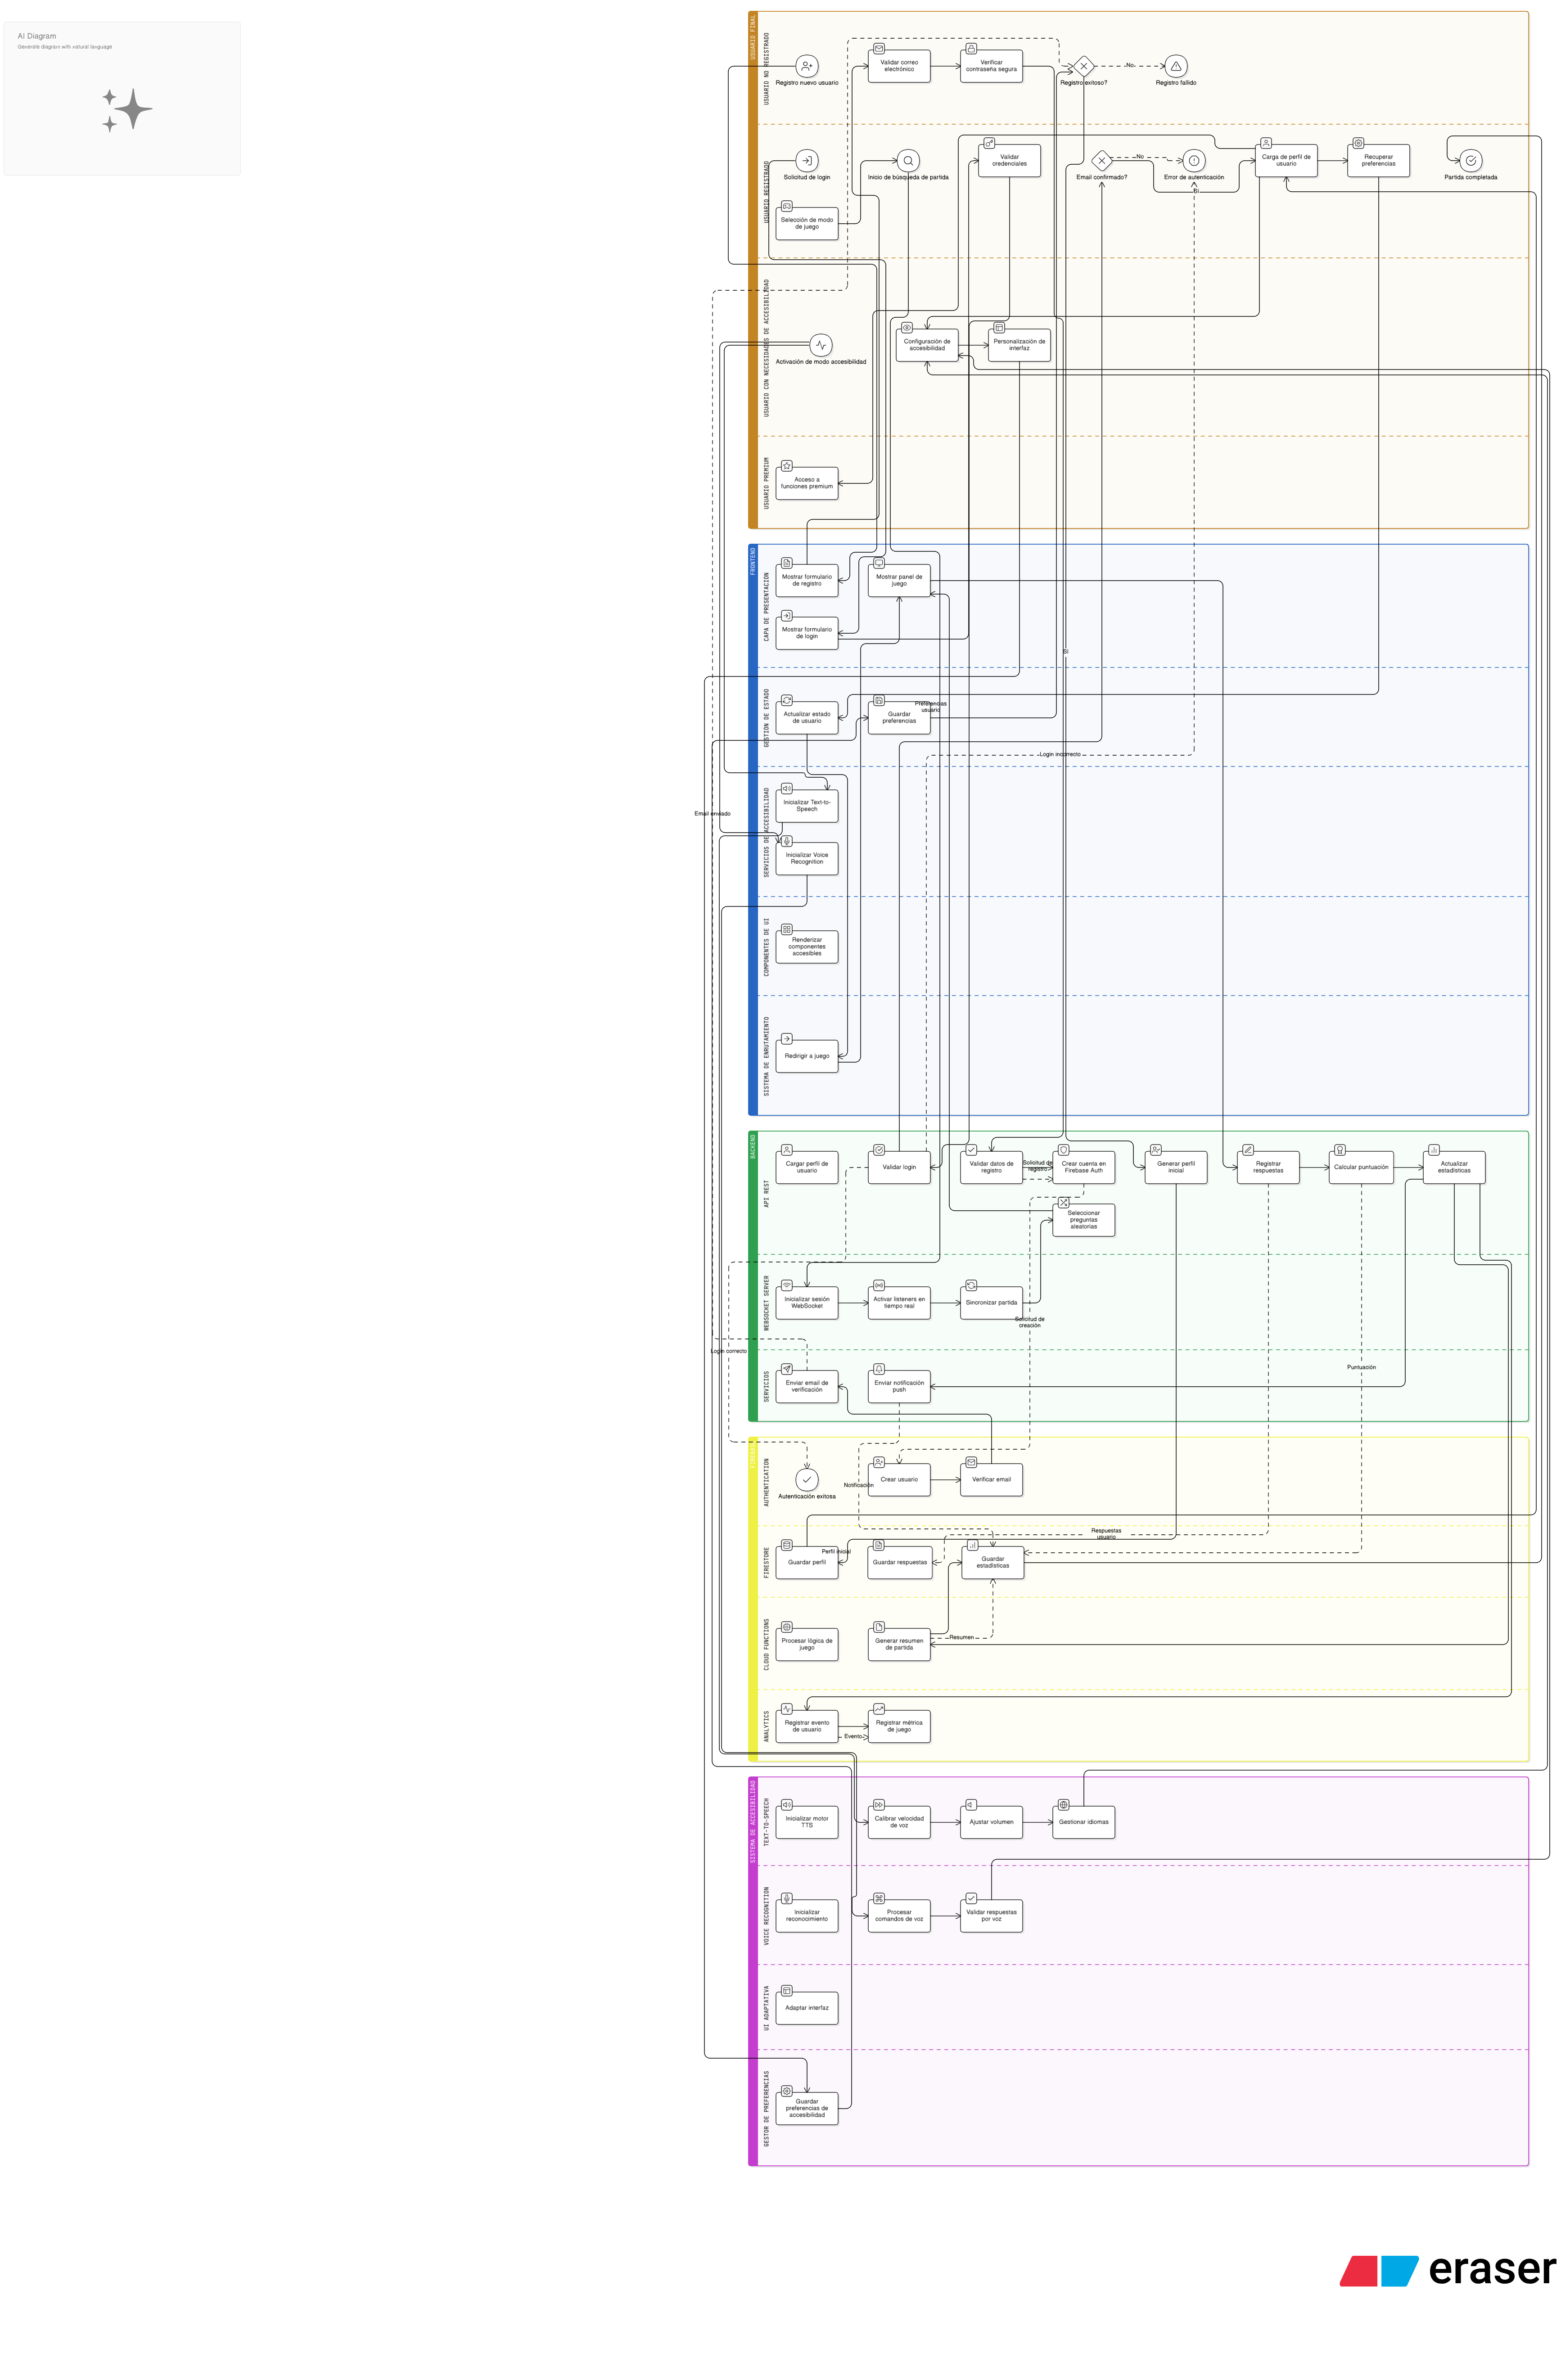
\includegraphics[width=0.8\textwidth]{diagrama BPMN.png}
    \caption{Diagrama BPMN del flujo de juego y accesibilidad}
\end{figure}

\subsection{Documentación completa del BPM}

% Inserted detailed BPM documentation provided by the project owner
\subsubsection*{Resumen ejecutivo}
BrainBlitz es una aplicación de juegos de trivia multijugador que incorpora características avanzadas de accesibilidad. A continuación se presenta la documentación completa del Business Process Model (BPM) que define la arquitectura y flujos de trabajo del sistema.

\paragraph{Propósito del documento}
Este BPM sirve como guía principal para la implementación técnica del sistema, la definición de flujos de trabajo, el establecimiento de estándares de calidad, la documentación de procesos de negocio y como base para futuras mejoras y escalabilidad.

\paragraph{Objetivos del sistema}
\begin{enumerate}
  \item Proporcionar una plataforma de juegos accesible.
  \item Garantizar una experiencia de usuario fluida.
  \item Mantener alta disponibilidad y rendimiento.
  \item Asegurar la integridad de los datos.
  \item Facilitar la escalabilidad del sistema.
\end{enumerate}

\paragraph{Alcance del proyecto}
Incluye: sistema completo de juego, gestión de usuarios, accesibilidad y análisis.\\
Excluye: integraciones de terceros no especificadas y sistemas externos.

\subsubsection*{Pools y lanes detallados}
La definición de pools y lanes permite mapear responsabilidades e interfaces entre actores y componentes técnicos del sistema. Se enumeran a continuación los pools y sus lanes principales tal como se documentaron:
\begin{itemize}
  \item \textbf{Usuario final}: Usuario No Registrado; Usuario Registrado; Usuario con Necesidades de Accesibilidad; Usuario Premium.
  \item \textbf{Frontend (React)}: Capa de Presentación; Gestión de Estado (Context API); Servicios de Accesibilidad; Componentes de UI; Sistema de Enrutamiento.
  \item \textbf{Backend (Node.js)}: API REST; WebSocket Server; Controladores; Middleware; Servicios; Utilidades.
  \item \textbf{Firebase}: Authentication; Firestore; Cloud Functions; Storage; Analytics.
  \item \textbf{Sistema de Accesibilidad}: Text-to-Speech; Voice Recognition; UI Adaptativa; Gestor de Preferencias.
\end{itemize}

\subsubsection*{Procesos principales con subprocesos}
Se identifican cuatro grandes áreas de procesos (Registro y autenticación, Sistema de accesibilidad, Sistema de juego y Administración y monitoreo), cada una con subprocesos que representan tareas concretas:
\paragraph{A. Registro y autenticación}
  \textbf{A.1 Registro de Usuario}: validación de correo, verificación de contraseña, creación de cuenta en Firebase Auth, generación de perfil inicial, configuración de preferencias y envío de email de verificación.

  \textbf{A.2 Inicio de sesión}: validación de credenciales, verificación de email, carga de perfil, recuperación de preferencias, inicialización de sesión WebSocket y activación de listeners en tiempo real.

  \textbf{A.3 Gestión de perfil}: actualización de datos personales, gestión de preferencias, historial de partidas, estadísticas de juego, logros y configuración de privacidad.

\paragraph{B. Sistema de accesibilidad}
  \textbf{B.1 Configuración inicial}: detección de necesidades, prueba del sistema de voz, calibración de velocidad de voz, ajuste de volumen, configuración de comandos de voz y personalización de interfaz.

  \textbf{B.2 Gestión de Text-to-Speech}: inicialización del motor TTS, cola de mensajes, priorización, control de interrupciones, gestión de idiomas y caché de audio.

  \textbf{B.3 Sistema de Voice Recognition}: inicialización del reconocimiento, procesamiento de comandos, validación de respuestas, gestión de errores, retroalimentación auditiva y modo de corrección.

\paragraph{C. Sistema de juego}
  \textbf{C.1 Preparación de partida}: selección de modo, búsqueda de jugadores, emparejamiento, sincronización inicial, carga de recursos y verificación de conexiones.

  \textbf{C.2 Gestión de preguntas}: selección aleatoria, validación de dificultad, formateo para accesibilidad, control de tiempo, registro de respuestas y análisis de patrones.

  \textbf{C.3 Sistema de puntuación}: cálculo de puntos base, bonificaciones por tiempo, multiplicadores, actualización en tiempo real, registro histórico y rankings.

  \textbf{C.4 Finalización de partida}: cálculo de resultados finales, actualización de estadísticas, asignación de experiencia, desbloqueo de logros, guardado de replay y generación de resumen.

\paragraph{D. Administración y monitoreo}
  extbf{D.1 Panel administrativo}: gestión de usuarios, moderación de contenido, control de acceso, configuración del sistema, gestión de recursos y reportes.

  extbf{D.2 Analytics y métricas}: seguimiento de usuarios activos, análisis de uso, métricas de accesibilidad, estadísticas de juego, reportes de rendimiento y KPIs.

  extbf{D.3 Mantenimiento}: respaldos automáticos, limpieza de datos, optimización de BD, actualización de contenido, gestión de caché y monitoreo de errores.

\subsubsection*{Eventos detallados}
Se definen eventos de inicio, intermedios, de error, de compensación y de finalización que guían la orquestación de procesos (p.ej. registro de usuario, temporizador de respuesta, fallo de conexión, recuperación de sesión, finalización de partida).

\subsubsection*{Compuertas lógicas}
Se documentan las compuertas exclusivas (decisiones binarias como validación de credenciales), inclusivas (selección de modos o configuraciones), paralelas (servicios inicializados en paralelo) y complejas (orquestación del flujo de juego y sistema de recompensas).

\subsubsection*{Flujos de datos detallados}
Incluye flujos de mensajes (cliente-servidor, WebSocket, notificaciones), flujos de secuencia (registro, juego, sincronización) y flujos de asociación que mapean relaciones entre entidades y servicios.

\subsubsection*{Actividades, artefactos y métricas}
Se enlistan tareas de usuario, tareas de servicio, scripts y reglas de negocio; los artefactos incluyen objetos de datos (perfiles, preguntas, logs), almacenes (Firestore, caché) y anotaciones (documentación técnica). Métricas y KPIs cubren usuario, sistema y negocio (tiempo de sesión, latencia, ROI, churn rate).

\subsubsection*{Requisitos técnicos, implementación y despliegue}
Se recogen requisitos de infraestructura (Node.js, Firebase, CDN, bases de datos), seguridad (autenticación, autorización, encriptación) y performance (latencia, throughput). La estrategia de despliegue considera pruebas, despliegue gradual, monitoreo y plan de migración con rollback.

\subsubsection*{Consideraciones de seguridad y plan de contingencia}
Incluye protección de datos, control de acceso, cumplimiento normativo, gestión de riesgos, recuperación de desastres y continuidad de negocio, con procedimientos de backup, restauración, pruebas y roles definidos.

\subsubsection*{Mapeo de historias de usuario}
Se presenta un mapeo entre HU y componentes del BPM: por ejemplo, HU-001 (Registro) enlaza con el pool Usuario Final y el proceso A.1; HU-002 (Inicio de sesión con accesibilidad) enlaza con el Sistema de Accesibilidad y A.2; HU-003 y HU-004 cubren preparación de partida y sistema de puntuación; HU-005 y HU-006 cubren configuración de voz y reconocimiento.

\subsubsection*{Flujos críticos e interacciones clave}
Se identifican y describen flujos críticos: ciclo de interacción por voz (latencia objetivo 200ms, sincronización TTS/STT), sincronización multiplayer (sub-segundo), integridad de datos (consistencia transaccional) y optimización de recursos (tiempo de respuesta objetivo <100ms).

\subsubsection*{Escenarios de manejo de errores y recuperación}
Se detalla la respuesta a desconexiones, fallos de voz, errores de sincronización con Firebase, corrupción de datos, intentos de acceso no autorizado, fallos de autenticación y sobrecargas. Cada escenario incluye pasos de detección, mitigación y restauración.

\paragraph{Apéndices}
La documentación incluye glosario, referencias y control de versiones. Se recomienda mantener este documento alineado con la implementación y actualizarlo periódicamente.


% Metodología Ágil
\section{Metodología Ágil (Scrum) aplicada al proyecto}
En este proyecto se adoptó un enfoque ágil basado en Scrum adaptado al alcance de un MVP académico. La implementación de Scrum se diseñó para encajar con los recursos y el calendario del curso. A continuación se documentan roles, ceremonias, artefactos, prácticas y métricas empleadas, con referencia explícita a las tareas y entregables técnicos del repositorio.

\subsection{Roles y responsabilidades}
- \textbf{Ervin Caravalí Ibarra (Backend, Product Owner y Scrum Master):} Según la organización del equipo y las contribuciones registradas, Ervin asumió la responsabilidad del desarrollo del backend (implementación de API, servicios de IA y voz, orquestación WebSocket) y simultáneamente actuó como Product Owner (PO) y Scrum Master (SM). Como PO definió y priorizó el Product Backlog, clarificó criterios de aceptación y mantuvo la visión del producto; como SM facilitó ceremonias, eliminó impedimentos y coordinó la entrega iterativa.
- \textbf{Compañeros (Frontend):} Los otros dos miembros del equipo se enfocaron en el desarrollo del frontend (implementación de la SPA en React, integración con servicios de voz, adaptación de UI y pruebas de accesibilidad). Su trabajo incluyó crear componentes, páginas, rutas y las integraciones con Firebase y el backend.

\subsection{Artefactos y gestión del backlog}
- \textbf{Product Backlog:} El backlog formal se generó a partir del análisis del repositorio y los prompts; contiene las HU (US1..US9) priorizadas y con estimaciones iniciales. El backlog fue el artefacto central para planificar sprints y asignar trabajo.
- \textbf{Sprint Backlog:} Para cada sprint (Sprint 1: 7-14 de octubre; Sprint 2: 15-21 de octubre) se seleccionaron las HU de mayor prioridad y se descompusieron en tareas técnicas: endpoints, controladores, servicios, componentes UI, pruebas y documentación. Cada tarea incluía criterios de aceptación y estimación en puntos de historia.
- \textbf{Definition of Done (DoD):} Se acordó que una tarea estaba "done" cuando: el código estaba integrado en la rama principal mediante pull request revisado, existían pruebas unitarias o de integración relevantes, la documentación mínima estaba actualizada (README o comentario en la HU) y el despliegue en staging pasaba las comprobaciones básicas.

\subsection{Ceremonias y cadencia}
- \textbf{Sprint Planning:} Antes de cada sprint se realizó (o se documentó) una planificación donde el PO presentaba las HU seleccionadas, se estimaban tareas y se asignaban responsables. El calendario de dos sprints cortos permitió iteraciones rápidas y foco en entregables funcionales.
- \textbf{Daily Stand-ups:} Se mantuvo una comunicación diaria (informal o mediante issues/commits) para reportar progreso, bloqueos y siguientes pasos. Como SM, Ervin recogía impedimentos relacionados con el backend, la integración de IA o la configuración de despliegue.
- \textbf{Sprint Review / Demo:} Al cierre de cada sprint se realizaron demos funcionales (o se dejaron evidencias en el repositorio con capturas/archivos) para validar las HU completadas frente a los criterios de aceptación.
- \textbf{Sprint Retrospective:} Se documentaron lecciones aprendidas y acciones de mejora (p. ej. mejorar definición de tareas, ajustar estimaciones, aumentar cobertura de pruebas, optimizar procesos de integración con servicios de IA).

\subsection{Planificación y asignación de tareas}
La planificación partió del Product Backlog generado por los prompts. Ervin lideró la definición técnica de las HU relacionadas con backend, IA y voz (US1, US3, US5, US8, US9), mientras que los desarrollos de UI y experiencia correspondieron a los compañeros (US2, US4, US6, US7). Para cada HU se documentaron notas de soporte indicando si la implementación debía realizarse en backend o frontend, lo que facilitó una separación clara de responsabilidades.

\subsection{Integración continua y control de calidad}
- \textbf{Control de versiones:} Se empleó GitHub para control de versiones; las ramas seguían una convención (por ejemplo hu-XXX-descripcion) para enlazar PRs con HU.
- \textbf{Pull Requests y revisión:} Las integraciones a la rama principal requerían PRs con descripción de cambios, referencia a la HU y revisión por al menos otro miembro. Como PO/SM, Ervin aprobaba las PRs de backend y verificaba que se cumpliera la DoD.
- \textbf{Pruebas automatizadas:} Se implementaron pruebas unitarias e integraciones básicas en backend y frontend; los scripts de pruebas y validación están en los directorios `tests/` y en los scripts del proyecto.
- \textbf{Pipelines y despliegue:} El pipeline de CI (documentado mediante scripts y \texttt{run\_all\_tests.sh}) ejecuta pruebas y validaciones; el despliegue final se realizó en Render con variables de entorno seguras y servicios gestionados para producción.

\subsection{Métricas y seguimiento}
- \textbf{Velocidad (Velocity):} Dado el calendario corto, la métrica de velocidad se registró en puntos por sprint para estimar la capacidad del equipo en iteraciones siguientes.
- \textbf{Burndown / Progreso:} Se utilizó el backlog y el historial de commits/PRs para medir el progreso y comparar con el plan original.
- \textbf{Calidad:} Métricas de cobertura de pruebas, número de incidencias abiertas y tiempo medio de resolución se emplearon para evaluar la salud del proyecto.

\subsection{Rol combinado de Product Owner y Scrum Master}
Combinar las funciones de PO y SM es una decisión frecuente en equipos pequeños o académicos. En este proyecto, Ervin equilibró la visión del producto y la priorización del backlog (PO) con la facilitación del proceso, la gestión de impedimentos y la coordinación (SM). Se documentan ventajas y riesgos:
\begin{itemize}
  \item \textbf{Ventajas:} velocidad de decisión, menor fricción en la priorización, conocimiento técnico profundo para resolver impedimentos.
  \item \textbf{Riesgos:} concentración de responsabilidades, posibilidad de sesgo en priorización técnica sobre necesidades de UX, carga de trabajo para el rol combinado.
\end{itemize}

\subsection{Lecciones aprendidas y recomendaciones}
Basado en la ejecución del proyecto se identifican las siguientes recomendaciones prácticas para futuros sprints o entregas:
\begin{itemize}
  \item Separar explícitamente tiempo para tareas de integración y pruebas de accesibilidad en cada sprint.
  \item Mantener un registro detallado de prompts y resultados para auditar decisiones de IA y mejorar reproducibilidad.
  \item Incrementar las pruebas automatizadas del flujo de voz (TTS/STT) y escenarios de error (latencia, desconexión).
  \item Delegar tareas de Product Owner cuando la carga de entrega crezca, para evitar cuellos de botella.
\end{itemize}


% Backend (Node.js, Express, Firebase)
\section{Backend (Node.js, Express, Firebase)}
El backend implementa la lógica de negocio, gestión de usuarios, partidas y preguntas, y funcionalidades de accesibilidad. Los modelos principales incluyen usuarios (con campo \texttt{visualDifficulty}), partidas, preguntas y registros de interacciones de voz. Ejemplo de registro de usuario con preferencia de accesibilidad:

El proceso de registro está diseñado para garantizar integridad y accesibilidad: al recibir la solicitud, el servidor valida el correo electrónico y la fortaleza de la contraseña, normaliza los campos de entrada y verifica la presencia del indicador de accesibilidad (campo booleano \texttt{visualDifficulty}).

Si la validación es correcta, el flujo crea la cuenta en el servicio de autenticación (Firebase Auth) y crea un documento de perfil en la colección de usuarios de Firestore. Este documento contiene campos iniciales de estado (estadísticas de juego, preferencias, nombre de usuario) y el flag de accesibilidad. En caso de error de validación, el servicio devuelve un código de estado 400 con mensaje descriptivo; si ocurre una excepción del sistema, se registra el error y se devuelve un 500.

La decisión de mantener la preferencia de accesibilidad en el perfil del usuario permite que, en el inicio de sesión, el frontend consulte esta preferencia y active automáticamente el modo de voz sin intervención adicional del usuario.

La API expone endpoints REST para registro, autenticación, gestión de partidas y preguntas, y funcionalidades de voz. La documentación completa está disponible en Swagger:
\begin{itemize}
    \item \texttt{POST /api/users/register} — Registrar usuario
    \item \texttt{GET /api/games} — Listar partidas
    \item \texttt{POST /api/questions} — Crear pregunta
    \item \texttt{POST /api/voice-interactions} — Registrar interacción de voz
    \item \texttt{GET /api/admin/accessibility} — Configuración de accesibilidad
\end{itemize}

El backend integra servicios de IA para generación de preguntas (Groq/OpenAI) y procesamiento de voz (Azure TTS, AssemblyAI). Ejemplo de generación de preguntas:
La generación de preguntas mediante IA está encapsulada en un servicio que construye prompts estructurados y realiza llamadas HTTP a proveedores (Groq, OpenAI). El servicio aplica validaciones sobre la respuesta recibida: asegura que el contenido sea JSON válido, que la estructura de preguntas cumpla con el esquema esperado (pregunta, opciones, respuesta correcta, metadatos de dificultad) y registra métricas de uso y latencia.

Se implementan mecanismos de tolerancia a fallos: si la primera API falla o devuelve contenido inválido, el servicio intenta un proveedor alternativo o retorna un error controlado para revisión manual. Además, las respuestas de IA se sujetan a reglas de moderación y formateo antes de ser persistidas en la base de datos.

% Frontend (React, Vite, TailwindCSS)
\section{Frontend (React, Vite, TailwindCSS)}
El frontend es una SPA moderna que consume la API y gestiona la experiencia de usuario. La estructura de carpetas incluye componentes, páginas, servicios y estilos. Ejemplo de integración de contexto de autenticación y voz:

La aplicación frontend está organizada en torno a providers y contextos que centralizan el estado de autenticación y las preferencias de accesibilidad (incluido el modo de voz). Esta arquitectura facilita el acceso global a la configuración de TTS, la cola de reproducción y los permisos de usuario desde cualquier componente de la interfaz.

La navegación se configura mediante un conjunto de rutas protegidas que habilitan o restringen el acceso según el estado de autenticación y el rol del usuario (p. ej. administrador). Las rutas clave incluyen las páginas de registro, inicio de sesión, dashboard, perfil, lobby y partida en tiempo real; cada una está diseñada para interactuar con la API a través de una capa de servicios que maneja autenticación, reintentos y control de errores.

% Prompts del desarrollo (IA aplicada al proyecto)
\section{Desarrollo y documentación de prompts}

\subsection{Prompts de backend}

\subsubsection{Prompt-Backend-1: Análisis inicial y planificación}
\begin{itemize}
    \item \textbf{Autor}: Ervin Caravali Ibarra
    \item \textbf{Objetivo}: Análisis exhaustivo del proyecto para generar documentación ágil
    \item \textbf{Mensaje del prompt}:
    \begin{verbatim}
READ THE ENTIRE PROJECT you have access to, including:
- backend-v1 (contains backend, database, APIs, and technical documentation).
- frontend-v2 (contains frontend, APIs, documentation, and configurations).

The functionality must mandatorily include:
- Option during user registration to indicate if they have visual difficulties.
- Backend field to store that preference.
- Automatic change in the frontend to "voice mode" if the user has this preference.
- Reading of questions via Text-to-Speech.
- Voice adjustments (voice, speed, volume).
- Storage of interaction history in voice mode.
- Accessible tutorial in audio format.
- Administrative control to configure accessibility.

GENERATE:
1° Eight User Stories (US) in CONESSA format with clear acceptance criteria.
2° Formal Product Backlog structured as a table.
3° Formal Release Plan (October 7-21) divided into two sprints.
    \end{verbatim}
    \item \textbf{Tiempo estimado}: 1 minuto 35 segundos
    \item \textbf{Archivos afectados}: Carpetas backend-v1 y frontend-v2
\end{itemize}

\subsubsection{Prompt-Backend-2: Workflow de HU completadas}
\begin{itemize}
    \item \textbf{Autor}: Ervin Caravali Ibarra
    \item \textbf{Objetivo}: Automatizar el paso de HU a "Done" al cerrar PR
    \item \textbf{Mensaje del prompt}:
    \begin{verbatim}
Create a GitHub Actions workflow called "Move HU to Done" that is triggered when 
a pull request is closed. The workflow must:
1. Extract the User Story (HU) number from the branch name (format: hu-XXX-name)
2. Verify that an issue with that number exists in the repository
3. If the PR was merged, move the HU to the "Done" column
4. Handle errors if the issue does not exist
    \end{verbatim}
    \item \textbf{Tiempo estimado}: 40 segundos
    \item \textbf{Archivo generado}: move-hu-done.yml
\end{itemize}

\subsubsection{Prompt-Backend-3: Workflow de HU en progreso}
\begin{itemize}
    \item \textbf{Autor}: Ervin Caravali Ibarra
    \item \textbf{Objetivo}: Automatizar el paso de HU a "In Progress"
    \item \textbf{Mensaje del prompt}:
    \begin{verbatim}
Create a GitHub Actions workflow called "Move HU to In Progress" that is triggered
when a pull request is opened or updated. The workflow must:
1. Extract the User Story (HU) number from the branch name
2. Verify that an issue with that number exists
3. Move the HU to the "In Progress" column
4. Handle errors appropriately
    \end{verbatim}
    \item \textbf{Tiempo estimado}: 40 segundos
    \item \textbf{Archivo generado}: move-hu-in-progress.yml
\end{itemize}

\subsubsection{Prompt-Backend-4: Inicialización de proyecto}
\begin{itemize}
    \item \textbf{Autor}: Ervin Caravali Ibarra
    \item \textbf{Objetivo}: Automatizar configuración inicial del proyecto
    \item \textbf{Mensaje del prompt}:
    \begin{verbatim}
Create a GitHub Actions workflow "Create Project Backlog and Sprints" that:
1. Check if the "Product Backlog" project exists
2. Create priority labels
3. Create milestones for backend and frontend sprints
4. Create issues for each user story
5. Add issues to project and move to "To Do"
6. Create and link branches
    \end{verbatim}
    \item \textbf{Tiempo estimado}: 1 minuto
    \item \textbf{Archivo generado}: product-backlog.yml
\end{itemize}

\subsubsection{Prompt-Backend-5: Integración WebSocket}
\begin{itemize}
    \item \textbf{Autor}: Ervin Caravali Ibarra
    \item \textbf{Objetivo}: Integrar modo de voz con WebSocket
    \item \textbf{Mensaje del prompt}:
    \begin{verbatim}
Analyze the backend architecture and WebSocket implementation. Your task is to:
1. Identify entry/exit points for voice events
2. Modify/create controllers for WebSocket voice events
3. Ensure robust, scalable integration
4. Update documentation with technical details
    \end{verbatim}
    \item \textbf{Tiempo estimado}: 1 minuto
    \item \textbf{Archivos generados}: hybridServer.js, voiceController.js, voiceService.js
\end{itemize}

\subsubsection{Prompt-Backend-6: Procesamiento de voz}
\begin{itemize}
    \item \textbf{Autor}: Ervin Caravali Ibarra
    \item \textbf{Objetivo}: Implementar validación de respuestas por voz
    \item \textbf{Mensaje del prompt}:
    \begin{verbatim}
Implement processing and validation of voice answers using AssemblyAI:
1. Create/update POST /api/voice-responses/validate endpoint
2. Integrate AssemblyAI for speech-to-text
3. Register validated interactions in history
4. Document the integration flow
    \end{verbatim}
    \item \textbf{Tiempo estimado}: 1 minuto
    \item \textbf{Archivos generados}: voiceResponses.js, assemblyAIService.js, voiceHistoryService.js
\end{itemize}

\subsection{Prompts de frontend}

\subsubsection{Prompt-Frontend-1: Preferencia de accesibilidad}
\begin{itemize}
    \item \textbf{Autor}: Frontend Senior Developer
    \item \textbf{Objetivo}: Implementar opción de accesibilidad en registro
    \item \textbf{Mensaje del prompt}:
    \begin{verbatim}
Implement an accessibility preference option in registration:
1. Add checkbox for "Tengo dificultades visuales"
2. Manage state and include in registration payload
3. Update API service to transmit field
4. Display confirmation of saved preference
5. Ensure accessibility best practices
6. Add/Update unit tests
    \end{verbatim}
    \item \textbf{Tiempo estimado}: 1 minuto 30 segundos
    \item \textbf{Archivos generados}: Register.jsx, api.js, Register.test.jsx
\end{itemize}

\subsubsection{Prompt-Frontend-2: Modo de voz automático}
\begin{itemize}
    \item \textbf{Autor}: Frontend Senior Developer
    \item \textbf{Objetivo}: Activar modo de voz automáticamente
    \item \textbf{Mensaje del prompt}:
    \begin{verbatim}
Implement automatic activation of "voice mode":
1. On login, fetch accessibility preference
2. If enabled, activate voice mode automatically
3. Provide UI toggle for manual control
4. Ensure toggle is accessible
5. Add tests for activation logic
    \end{verbatim}
    \item \textbf{Tiempo estimado}: 1 minuto 30 segundos
    \item \textbf{Archivos generados}: AuthContext.jsx, VoiceContext.jsx, VoiceToggle.jsx
\end{itemize}

\subsubsection{Prompt-Frontend-3: Text-to-Speech}
\begin{itemize}
    \item \textbf{Autor}: Frontend Senior Developer
    \item \textbf{Objetivo}: Implementar lectura TTS de preguntas
    \item \textbf{Mensaje del prompt}:
    \begin{verbatim}
Implement Text-to-Speech for questions:
1. Integrate TTS in question component
2. Add play/pause/resume/stop controls
3. Read question and options clearly
4. Allow repeat functionality
5. Ensure control accessibility
6. Add test coverage
    \end{verbatim}
    \item \textbf{Tiempo estimado}: 1 minuto 30 segundos
    \item \textbf{Archivos generados}: Question.jsx, TTSControls.jsx, TTS.test.jsx
\end{itemize}

\subsubsection{Prompt-Frontend-4: Configuración de voz}
\begin{itemize}
    \item \textbf{Autor}: Frontend Senior Developer
    \item \textbf{Objetivo}: Implementar panel de ajustes de voz
    \item \textbf{Mensaje del prompt}:
    \begin{verbatim}
Create voice settings panel:
1. UI for voice parameters
2. Voice/speed/volume controls
3. Settings persistence
4. Real-time preview
5. Accessibility compliance
6. Test coverage
    \end{verbatim}
    \item \textbf{Tiempo estimado}: 1 minuto 30 segundos
    \item \textbf{Archivos generados}: VoiceSettings.jsx, VoiceContext.jsx, VoiceSettings.test.jsx
\end{itemize}

\subsubsection{Prompt-Frontend-5: Historial de voz}
\begin{itemize}
    \item \textbf{Autor}: Frontend Senior Developer
    \item \textbf{Objetivo}: Mostrar historial de interacciones
    \item \textbf{Mensaje del prompt}:
    \begin{verbatim}
Create voice interaction history view:
1. Display history in accessible table
2. Show date, question, response, result
3. Handle loading/empty/error states
4. Ensure responsive design
5. Add test coverage
    \end{verbatim}
    \item \textbf{Tiempo estimado}: 1 minuto 30 segundos
    \item \textbf{Archivos generados}: VoiceHistory.jsx, api.js, VoiceHistory.test.jsx
\end{itemize}

\subsubsection{Prompt-Frontend-6: Tutorial de audio}
\begin{itemize}
    \item \textbf{Autor}: Frontend Senior Developer
    \item \textbf{Objetivo}: Crear tutorial accesible en audio
    \item \textbf{Mensaje del prompt}:
    \begin{verbatim}
Implement audio tutorial:
1. Auto-trigger for new users
2. Cover key features
3. Add pause/resume/skip controls
4. Enable replay functionality
5. Ensure accessibility
    \end{verbatim}
    \item \textbf{Tiempo estimado}: 1 minuto 30 segundos
    \item \textbf{Archivos generados}: AudioTutorial.jsx, VoiceContext.jsx, AudioTutorial.test.jsx
\end{itemize}

\subsubsection{Prompt-Frontend-7: Panel administrativo}
\begin{itemize}
    \item \textbf{Autor}: Frontend Senior Developer
    \item \textbf{Objetivo}: Implementar controles de accesibilidad admin
    \item \textbf{Mensaje del prompt}:
    \begin{verbatim}
Add admin accessibility controls:
1. Create dedicated section
2. Enable/disable feature toggles
3. Persist configuration
4. Ensure panel accessibility
5. Add test coverage
    \end{verbatim}
    \item \textbf{Tiempo estimado}: 1 minuto 30 segundos
    \item \textbf{Archivos generados}: AdminPanel.jsx, AccessibilityControls.jsx, AdminPanel.test.jsx
\end{itemize}

\subsubsection{Prompt-Frontend-8: Integración modo de voz}
\begin{itemize}
    \item \textbf{Autor}: Frontend Senior Developer
    \item \textbf{Objetivo}: Integrar modo de voz con juego
    \item \textbf{Mensaje del prompt}:
    \begin{verbatim}
Implement voice mode integration:
1. Support all game interactions
2. Provide clear feedback
3. Handle edge cases
4. Adapt UI dynamically
5. Add integration tests
    \end{verbatim}
    \item \textbf{Tiempo estimado}: 1 minuto 30 segundos
    \item \textbf{Archivos generados}: VoiceContext.jsx, Game.jsx, VoiceGame.test.jsx
\end{itemize}

\subsubsection{Prompt-Frontend-9: Reconocimiento de voz}
\begin{itemize}
    \item \textbf{Autor}: Frontend Senior Developer
    \item \textbf{Objetivo}: Implementar respuestas por voz
    \item \textbf{Mensaje del prompt}:
    \begin{verbatim}
Implement voice recognition:
1. Integrate Web Speech API
2. Connect to answer validation
3. Provide real-time feedback
4. Ensure accessibility
5. Add recognition tests
    \end{verbatim}
    \item \textbf{Tiempo estimado}: 1 minuto 30 segundos
    \item \textbf{Archivos generados}: VoiceRecognition.jsx, VoiceContext.jsx, VoiceRecognition.test.jsx
\end{itemize}


\section{Product Backlog y Release Plan}

\subsection{Product Backlog}
El Product Backlog se ha estructurado cuidadosamente considerando las prioridades del proyecto y la dependencia entre historias de usuario:

\clearpage
\begin{table}[!htbp]
\centering
\footnotesize
\caption{Product Backlog del Proyecto}
\begin{tabular}{@{}l p{0.22\textwidth} c c p{0.15\textwidth} c p{0.2\textwidth}@{}}
	oprule
	extbf{ID} & \textbf{Historia} & \textbf{Prio.} & \textbf{SP} & \textbf{Resp.} & \textbf{Ubic.} & \textbf{Notas} \\
\midrule
US1 & Registro de preferencia de accesibilidad & Alta & 3 & Dev Backend & BE & Campo \texttt{visualDifficulty} en usuarios \\
US2 & Activación auto. modo voz & Alta & 5 & Dev Frontend & FE & Modificar AuthContext.jsx \\
US3 & Lectura TTS de preguntas & Alta & 8 & Dev Frontend & FE & Web Speech API \\
US4 & Config. ajustes de voz & Media & 5 & Dev Frontend & FE & Componente ajustes \\
US5 & Historial interacciones & Media & 6 & Dev Backend & BE & Colección \texttt{voiceInteractions} \\
US6 & Tutorial de audio & Media & 7 & Dev Frontend & FE & Componente tutorial \\
US7 & Config. admin accesibilidad & Baja & 4 & Dev Backend & BE & AdminPage.jsx \\
US8 & Integración modo voz & Alta & 6 & Dev Frontend & FE & WebSocket \\
US9 & Reconocimiento voz & Alta & 10 & Dev FE + BE & FE+BE & Web Speech + Backend \\
\bottomrule
\end{tabular}
\label{tab:product-backlog}
\end{table}

\subsection{Plan de Lanzamiento (7-21 de Octubre)}

\subsubsection{Estrategia: Backend Primero}
La estrategia adoptada es "Backend Primero", lo que significa que el backend debe estar completamente terminado antes de que el frontend comience a trabajar. Esto asegura que todas las APIs y funcionalidades estén listas cuando los desarrolladores frontend las necesiten.

\subsubsection{Sprint Backend (7-15 de Octubre): Infraestructura Completa}
\textbf{Objetivo}: Completar TODAS las funcionalidades de backend antes de que el frontend comience.

\textbf{Historias de Usuario Backend Asignadas}:
\begin{itemize}
    \item US1: Registro de preferencia de accesibilidad (3SP)
    \item US5: Almacenamiento del historial de interacciones de voz (6SP)
    \item US7: Configuración administrativa de accesibilidad (4SP)
    \item US8: Integración del modo de voz con el juego (6SP)
    \item US9: Procesamiento y validación de respuestas por voz (4SP)
\end{itemize}

\textbf{Total de Story Points Backend}: 23SP

\subsubsection{Sprint Frontend (16-21 de Octubre): Implementación de UI/UX}
\textbf{Objetivo}: Implementar todas las funcionalidades frontend usando las APIs del backend ya terminadas.

\textbf{Historias de Usuario Frontend Asignadas}:
\begin{itemize}
    \item US1: Integración frontend de preferencia de accesibilidad (2SP)
    \item US2: Activación automática del modo de voz (5SP)
    \item US3: Lectura de preguntas mediante Text-to-Speech (8SP)
    \item US4: Configuración de ajustes de voz (5SP)
    \item US5: Integración frontend del historial de voz (3SP)
    \item US6: Sistema de tutorial de audio (7SP)
    \item US7: Panel administrativo frontend (2SP)
    \item US8: Integración frontend del modo de voz (3SP)
    \item US9: Reconocimiento de voz con Web Speech API (6SP)
\end{itemize}

	extbf{Total de Story Points Frontend}: 41SP

\subsection{Implementación y Seguimiento}

Las historias de usuario se implementarán siguiendo un enfoque sistemático basado en los sprints definidos. Cada historia tiene asignados responsables claros y criterios de aceptación específicos.

\subsubsection{Criterios de Éxito}
\begin{itemize}
    \item Backend completado antes del 16 de octubre
    \item Documentación Swagger actualizada
    \item Pruebas unitarias con cobertura >90\%
    \item Integración exitosa frontend-backend
    \item Rendimiento WebSocket sin degradación
\end{itemize}


% Product Backlog y Release Plan


% Despliegue e infraestructura
\section{Despliegue e infraestructura}
El sistema se despliega en la plataforma Render, utilizando una arquitectura distribuida:

\subsection{Servicios desplegados}
\begin{itemize}
    \item \textbf{Backend}: Servicio Node.js + Express desplegado en \url{https://proyecto-2-olvb.onrender.com/}
    \item \textbf{Frontend}: Aplicación React desplegada en \url{https://proyecto-2-2.onrender.com/}
    \item \textbf{Base de datos}: Firebase Firestore para almacenamiento de datos
    \item \textbf{Autenticación}: Firebase Auth para gestión de usuarios
\end{itemize}

\subsection{Configuración y gestión}
\begin{itemize}
    \item \textbf{Variables de entorno}: Gestión segura de credenciales de Firebase y claves de API
    \item \textbf{Integración continua}: Despliegue automático desde GitHub a Render
    \item \textbf{Monitorización}: Logs y métricas a través del dashboard de Render
    \item \textbf{Backup}: Respaldos automáticos gestionados por Firebase
\end{itemize}

\subsection{Flujo de despliegue}
1. Los cambios se integran mediante pull requests en GitHub
2. Las pruebas automatizadas se ejecutan en el pipeline de CI
3. Al aprobar y mergear, Render detecta los cambios
4. Se construye y despliega la nueva versión
5. Se verifican los endpoints de salud

% Resultados y conclusiones
\section{Resultados y conclusiones}
El proyecto BrainBlitz ha logrado implementar funcionalidades avanzadas de accesibilidad, integrando IA y tecnologías modernas para ofrecer una experiencia inclusiva y escalable. Se han cumplido los objetivos propuestos, y el sistema demuestra rendimiento y estabilidad en producción. Entre las mejoras futuras se propone ampliar el soporte multilingüe, optimizar el reconocimiento de voz y fortalecer la seguridad de datos.



% --------------------------------------------------
% Secciones añadidas para ampliar el informe (contratos, criterios, pruebas, plantillas)
% --------------------------------------------------

\section{Contratos y especificaciones de endpoints}
En esta sección se documentan de forma textual y académica los contratos principales expuestos por la API, describiendo entradas, salidas y modos de error. La finalidad es proporcionar una especificación legible por desarrolladores y por herramientas de prueba automatizadas.

\subsection{Registro de usuario — POST /api/users/register}
Entrada esperada: objeto JSON con campos de autenticación y perfil (correo, contraseña, nombre, preferencias de accesibilidad). El campo de preferencia de accesibilidad se modela como booleano \texttt{visualDifficulty} y determina el comportamiento por defecto en el frontend.

Salida satisfactoria: 201 Created con un objeto perfil que incluye identificador único, timestamp de creación y la preferencia de accesibilidad registrada. Errores esperados: 400 Bad Request (validación de datos), 409 Conflict (correo ya registrado), 500 Internal Server Error (falla de servicio externo).

Criterios de calidad: validación de formato de correo, comprobación de fortaleza de contraseña, sanitización de entradas y registro de auditoría para eventos críticos.

\subsection{Gestión de partidas — GET /api/games, POST /api/games}
GET /api/games devuelve una lista paginada de partidas disponibles o recientes; incluye filtros opcionales (estado, jugadores, modo). POST /api/games crea una nueva sesión con parámetros de configuración (modo de accesibilidad, límite de jugadores, temporizador).

Respuesta: en ambos casos se devuelve en el cuerpo JSON normalizado con metadatos de paginación para GET y objeto de recurso para POST. Errores: 401 Unauthorized si el token es inválido, 422 Unprocessable Entity si faltan parámetros obligatorios.

\subsection{Interacciones de voz — POST /api/voice-interactions}
Este endpoint centraliza el registro y persistencia de eventos relacionados con TTS/STT: inicio de reproducción, transcripción recibida, validación de respuesta y métricas de latencia. Entrada: objeto que describe tipo de evento, identificador de usuario, identificador de partida y payload del evento.

Salida: 200 OK con confirmación de registro. Es crítico que la latencia y el tamaño del payload estén controlados para evitar sobrecarga; por ello se definen límites y validaciones en el gateway.

\section{Criterios de aceptación detallados por Historia de Usuario (HU)}
A continuación se amplían los criterios de aceptación por cada HU principal, expresados en lenguaje verificable y con condiciones de prueba.

\clearpage
\begin{table}[!htbp]
\centering
\footnotesize
\caption{Criterios de aceptación por Historia de Usuario}
\begin{tabular}{@{}p{1.5cm} p{8cm} p{5cm}@{}}
	oprule
	extbf{ID} & \textbf{Criterio de aceptación} & \textbf{Métrica / Validación} \\
\midrule
US1 & Al registrarse, el sistema almacena el flag \texttt{visualDifficulty} y el usuario ve el estado activo del modo de voz tras iniciar sesión. & Revisión: prueba manual + test de integración que verifica campo en Firestore; Must: campo existe y frontend activa TTS. \\
US2 & Si el usuario tiene \texttt{visualDifficulty} true, al iniciar sesión se activa la reproducción automática de instrucciones por TTS. & Test e2e que simula login y verifica llamada al servicio TTS y reproducción. \\
US3 & Las preguntas generadas por IA cumplen el esquema (enunciado, opciones, respuesta correcta, dificultad). & Validación automática sobre el payload JSON generado por el servicio de IA; rechazo y logging si no cumple. \\
US4 & El usuario puede ajustar velocidad y volumen del TTS desde configuración y estos parámetros se aplican en las partidas. & Prueba manual + test de integración que pasa parámetros y valida efecto en la respuesta del motor TTS (simulado). \\
US5 & Todas las interacciones de voz quedan registradas en la colección \texttt{voiceInteractions} con timestamps y latencias. & Auditoría de logs y test de integración que envía eventos y comprueba persistencia. \\
US6 & El tutorial de audio se reproduce correctamente y se puede reiniciar por el usuario. & Test funcional que invoca endpoint de tutorial y valida estado reproducido. \\
US7 & Un administrador puede actualizar configuraciones globales de accesibilidad desde el panel y las actualizaciones se propagan en tiempo real. & Test de integración con WebSocket que valida recepción de eventos de configuración. \\
US8 & El modo de voz se integra con el flujo de juego: preguntas, temporizador y respuestas por voz sincronizadas sin desincronización mayor a 200ms. & Prueba de rendimiento y medición de latencia; objetivo sub-200ms en condiciones nominales. \\
US9 & El reconocimiento de respuestas por voz acepta sinónimos y errores menores, aplicando reglas de tolerancia definidas. & Test de NLP con corpus de sinónimos; tasa de reconocimiento aceptable >= 85\%. \\
\bottomrule
\end{tabular}
\label{tab:criterios-aceptacion}
\end{table}

\section{Estrategia de pruebas y validación}
Se describe la estrategia completa de pruebas aplicada en el proyecto, organizadas por nivel y con criterios de aceptación cuantificados.

\subsection{Pruebas unitarias}
Cobertura objetivo: las unidades críticas del backend (generación y parsing de prompts, validaciones de payload, cálculo de puntuaciones) deben alcanzar al menos 70\% de cobertura. Las pruebas se diseñan para ejecutarse en CI con mocks de servicios externos (IA, TTS).

\subsection{Pruebas de integración}
Se verifican las interacciones entre servicios: API <-> Firestore, API <-> servicios de IA, API <-> motor TTS. Las pruebas usan entornos de staging con datos de prueba y client libraries configuradas para admitir reintentos y latencia simulada.

\subsection{Pruebas end-to-end (E2E)}
Se automatizan los flujos principales (registro, inicio de sesión con accesibilidad, creación y finalización de partida) mediante Playwright. Los E2E validan además la integración de TTS/STT mediante stubs que simulan los proveedores en CI.

\subsection{Pruebas de rendimiento}
Se planifican pruebas con carga creciente sobre el servidor de partidas para medir: latencia media, percentiles 95/99, throughput y tasa de fallos. Objetivo: mantener latencia de sync < 500ms para p95 y <1000ms para p99 bajo carga objetivo.

\subsection{Pruebas de accesibilidad}
Se realizan auditorías con herramientas automáticas (axe-core) y pruebas manuales con usuarios que requieran soporte de voz. Se documentan fallos y se priorizan en el backlog.

\section{Plantillas y buenas prácticas para issues y Pull Requests}
Se incorpora un modelo mínimo de PR y issue para asegurar la trazabilidad entre HU y cambios de código.

\subsection{Plantilla de Issue (Resumen)}
Cada issue debe contener: resumen claro, HU asociada (si aplica), pasos para reproducir (si es bug), resultado esperado, entorno y etiquetas (bug/feature/infra). Prioridad y estimación deben asignarse por el PO.

\subsection{Plantilla de Pull Request (Resumen)}
Un PR debe incluir: descripción del cambio, HUs relacionadas, checklist de DoD (tests añadidos/actualizados, documentación, revisión de seguridad), capturas si aplica y notas de despliegue.

\section{Métricas de calidad y seguimiento}
Las métricas clave definidas para evaluar el proyecto incluyen:
\begin{itemize}
  \item Cobertura de pruebas (unitarias e integración)
  \item Tiempo medio de resolución de incidencias
  \item Latencia media de TTS/STT y percentiles p95/p99
  \item Tasa de aciertos del reconocimiento de voz
  \item Velocidad del equipo (puntos por sprint)
\end{itemize}

Estas métricas se recolectan a través de pipelines y paneles de monitoring (por ejemplo, Grafana/Prometheus o soluciones gestionadas), y se revisan periódicamente en retrospectivas.

\section{Plan de despliegue extendido y rollback}
Se define una estrategia de despliegue segura: despliegues canary en staging, pruebas automáticas del release candidate, despliegue gradual a producción y monitorización inmediata. En caso de regresión crítica, se ejecuta rollback a la versión anterior del contenedor y se abre incidencia con prioridad alta para análisis forense.

\section{Anexos}
\subsection{Glosario}
Incluye términos técnicos usados en el informe: TTS (Text-to-Speech), STT (Speech-to-Text), DoD, HU (Historia de Usuario), CI/CD, p95/p99, etc.

\subsection{Evidencia de pruebas}
Se adjunta en el repositorio la salida de pruebas automáticas y logs esenciales; en el anexo se describe cómo localizar estos artefactos en `backend-v1/tests/reports` y `frontend-v2/playwright-report`.


\vfill

% Referencias y anexos
\section{Referencias y anexos}
\begin{itemize}
    \item Repositorio: \url{https://github.com/ErvinCaraval/PROYECTO-2}
    \item Backend desplegado: \url{https://proyecto-2-olvb.onrender.com/}
    \item Frontend desplegado: \url{https://proyecto-2-2.onrender.com/}
    \item Swagger API: \url{https://proyecto-2-olvb.onrender.com/api-docs}
    \item Bibliografía: \url{https://react.dev/}, \url{https://nodejs.org/}, \url{https://firebase.google.com/}, \url{https://docs.docker.com/}, \url{https://swagger.io/}
\end{itemize}

\end{document}
